\documentclass[a4paper, 12pt]{article}

\usepackage[T1]{fontenc}
\usepackage[utf8]{inputenc}
\usepackage[spanish, mexico]{babel}
\usepackage[style=mexican]{csquotes}
\usepackage[margin=2cm,top=2cm,includefoot]{geometry}
\usepackage[spanish, ruled, linesnumbered, lined]{algorithm2e}
\usepackage{amsmath, amsfonts, amssymb, amsthm, amsbsy, cancel}
\usepackage{microtype, parskip}
\usepackage{float, graphicx, subcaption}
\usepackage{circuitikz, tikz, pgfplots}
\usepackage{xcolor}
\usepackage{array, booktabs, multicol, multirow, tabularx}
\usepackage{hyperref, url}
\usepackage{siunitx}
\usepackage{tcolorbox}
\usepackage[style=ieee]{biblatex}
%definir el estilo de lapagina
\usepackage{fancyhdr}
%code
\usepackage{listings}


%variables de color
% \definecolor{greenPortada}{HTML}{69A84F}
%\definecolor{lineCabecera}{HTML}{5DADE2}
\definecolor{lineCabecera}{HTML}{008080}
%\definecolor{lineCabecera}{HTML}{FF4500}



%cabecera
\setlength{\headheight}{40pt}
\pagestyle{fancy}
\fancyhf{}
\renewcommand{\headrulewidth}{3pt}
\renewcommand{\headrule}{\hbox to \headwidth{\color{lineCabecera}\leaders\hrule height \headrulewidth\hfill}}

%variables globales
\newcommand{\control}{img/control.jpg}
\newcommand{\conjuntoD}{img/conjutodifuso.png}
\newcommand{\funcionM}{img/funcionM.png}
\newcommand{\fuzzy}{img/variableFuzzy.jpeg}
\newcommand{\imgA}{img/diag1.png}
\newcommand{\imgB}{img/diag2.png}


\newcommand{\codeA}{code/fuzzyS.m}





%gestion de hipervinculos
\hypersetup{
    breaklinks=true,
    colorlinks=true,
    citecolor=black,
    filecolor=magenta,
    linkcolor=black, 
    urlcolor=cyan
}
%gestor de codigo
\lstset{
    language=Matlab,
    basicstyle=\ttfamily,
    keywordstyle=\color{blue},    % Color de las palabras clave
    commentstyle=\color{green},   % Color de los comentarios
    numberstyle=\tiny\color{gray},% Color de los números de línea
    stringstyle=\color{red},      % Color de las cadenas de texto
    breaklines=true,
    numbers=left,
    frame=single,
}

\title{Control difuso}
\author{Universidad Nacional Autónoma de México.\\Facultad de Estudios Superiores Cuatitlán.\\Palomino Alfonso Edgar.\\Vargas Gachuz Alonso}
\date{\today}

\cfoot{\thepage}

\begin{document}
    \maketitle 
    \begin{abstract}
        El sistema propuesto en este informe se diseñó para gestionar motores que simulan salidas del mundo real mediante el procesamiento de datos provenientes de un sensor de temperatura y de luz. Estos sensores capturan información del entorno físico, permitiéndonos definir los parámetros del control utilizando lógica difusa. El sistema responde a las preferencias del usuario respecto a condiciones ambientales, como frío, calor o exceso de luz.
        La solución al problema se aborda mediante la interacción entre el medio físico y la tarjeta de adquisición de datos, en este caso, la tarjeta Arduino 1. La programación se realiza utilizando Matlab, aprovechando las librerías "Deep Learning" y "Fuzzy Logic Toolbox". Estas herramientas proporcionan un entorno de programación que facilita la implementación del sistema, un aspecto que se puede  destacar en este sistema es su capacidad de adaptación. Se pueden añadir o quitar entradas y variables según las necesidades específicas o cambios en el plan de funcionamiento. Esta versatilidad lo hace aplicable a diversas situaciones.        
    \end{abstract} 
    \vspace{2ex}

    \section{Introducción.}
    La automatización en el hogar o el mundo en general se ha dado de manera paulatina con una tendencia al aumento, debido a esto es que en la actualidad podemos hacer uso de herramientas que ayudan a facilitar la implementación de diferentes sistemas o hardware sobre un problema específico, es decir la particularización de los sistemas, si bien como se dijo se ha facilitado la implementación se requiere un cierta curva de aprendizaje al hacer uso de las herramientas, el presente trabajo se enfoca en el desarrollo de un sistema de control de diferentes salidas basado en lógica difusa. Este enfoque se selecciona en respuesta a la creciente necesidad de sistemas que puedan ajustarse dinámicamente a las condiciones ambientales cambiantes.
    La gestión de motores en entornos variables, como los influenciados por factores climáticos, representa un desafío significativo e importante en diferentes ámbitos de la vida. La elección de utilizar lógica difusa se fundamenta en su capacidad para manejar la imprecisión inherente a las entradas del mundo real, como la temperatura y la luz. Este enfoque no solo permite una adaptación más efectiva a las preferencias del usuario en términos de condiciones ambientales deseadas, como frío, calor o niveles de luz, sino que también ofrece flexibilidad para modificar el sistema según las necesidades específicas, esto nos permite la gestión eficiente de actuadores en entornos industriales hasta su implementación en sistemas domésticos, la capacidad de adaptación y la precisión en la respuesta del sistema tienen implicaciones significativas en términos de eficiencia energética y comodidad del usuario. Este enfoque busca no solo resolver un problema técnico específico, sino también contribuir a la creciente demanda de sistemas de control más inteligentes y adaptables en diversos contextos.

    %conocimientosP
    \section{Conocimientos previos.}
    Los conocimientos previos necesarios se centra sobre el conocimiento del control difuso como tal, aunque se requiere más que esto, como se mencionó antes la implementación es sencilla pero se debe de tener una noción previa de Arduino, de Matlab y de electrónica básica, esto en conjunto es lo que nos permite llevar  a cabo todo el sistema.


    \subsection{Lógica difusa.}
    La lógica difusa, también conocida como lógica borrosa, es un paradigma de lógica que difiere de la lógica clásica al manejar la imprecisión y la incertidumbre en la toma de decisiones. A diferencia de la lógica convencional que utiliza valores de verdad binarios (verdadero o falso), la lógica difusa utiliza conjuntos difusos y grados de membresía para representar y procesar la incertidumbre en los datos. Esta metodología permite modelar y controlar sistemas en los que las fronteras entre las categorías no son claramente definidas, haciendo que sea especialmente útil en situaciones donde las relaciones son complejas o ambiguas. La lógica difusa encuentra aplicaciones en una amplia variedad de campos, desde sistemas de control y procesamiento de señales hasta inteligencia artificial y toma de decisiones en entornos complejos delimitados. 

    \subsection{Conjuntos borrosos}
    Los conjuntos borrosos, también conocidos como conjuntos difusos, son una parte fundamental de la lógica difusa y se utilizan para representar la imprecisión y la incertidumbre en la toma de decisiones. A diferencia de los conjuntos clásicos en los que un elemento pertenece o no pertenece al conjunto de manera precisa, los conjuntos borrosos permiten que un elemento tenga un grado de pertenencia entre 0 y 1.
    En un conjunto borroso, la función de membresía asigna a cada elemento un valor que indica en qué medida pertenece al conjunto. Este enfoque es especialmente útil cuando se trata de conceptos lingüísticos o variables que no pueden clasificarse de manera estricta. La representación borrosa permite capturar la naturaleza subjetiva y vaga de la información, haciendo que sea más fácil modelar y controlar sistemas en los que la precisión no es posible o es limitada.
    La teoría de conjuntos borrosos ha demostrado ser valiosa en una amplia gama de aplicaciones, desde control de sistemas y procesamiento de señales hasta toma de decisiones en entornos complejos, donde la ambigüedad y la falta de información precisa son comunes. Este enfoque brinda flexibilidad y adaptabilidad en situaciones donde la rigidez de los conjuntos clásicos podría ser insuficiente.\\
    \emph{Definición}
    Sea $X$ una colección de objetos, expresados en forma genérica por $x$. Entonces,un conjunto difuso A en $X$,se define como un conjunto de pares ordenados.

    \begin{equation}
        A = \{ ( x,\mu_{A(x)} )/x \in X \}
    \end{equation}

    Donde $\mu_{A(x)}$ es una función de pertenencia cuya etiqueta es A y su dominio es $x$
    .
    \begin{figure}[H]
        \centering
        \includegraphics[width=0.8 \linewidth]{\conjuntoD}
        \caption{Conjuntos difusos}
        \label{fig:conjuntoD}
    \end{figure}

    \subsection{Función de membresía}
    La función de membresía es una herramienta esencial en la teoría de conjuntos borrosos y se utiliza para asignar un grado de pertenencia a un elemento en un conjunto difuso. Mientras que en la teoría de conjuntos clásica un elemento puede pertenecer completamente o no pertenecer en absoluto a un conjunto, la función de membresía permite una transición gradual entre la pertenencia y la no pertenencia.
    Esta función asigna a cada elemento un valor entre 0 y 1, indicando el grado en que el elemento pertenece al conjunto difuso. Por ejemplo, en un conjunto difuso que representa la categoría "altura baja", un individuo de estatura intermedia tendría un valor de membresía que reflejaría su grado de pertenencia a esa categoría.
    La forma específica de la función de membresía puede variar según el contexto y la naturaleza de la variable que se está modelando. Algunos tipos comunes de funciones de membresía incluye funciones triangulares, trapezoidales y gaussianas. Estas funciones permiten una representación más flexible y matizada de la incertidumbre y la imprecisión en situaciones del mundo real. La función de membresía es esencial para el cálculo y la interpretación de las operaciones lógicas en los sistemas basados en lógica difusa.

    \begin{figure}[H]
        \centering
        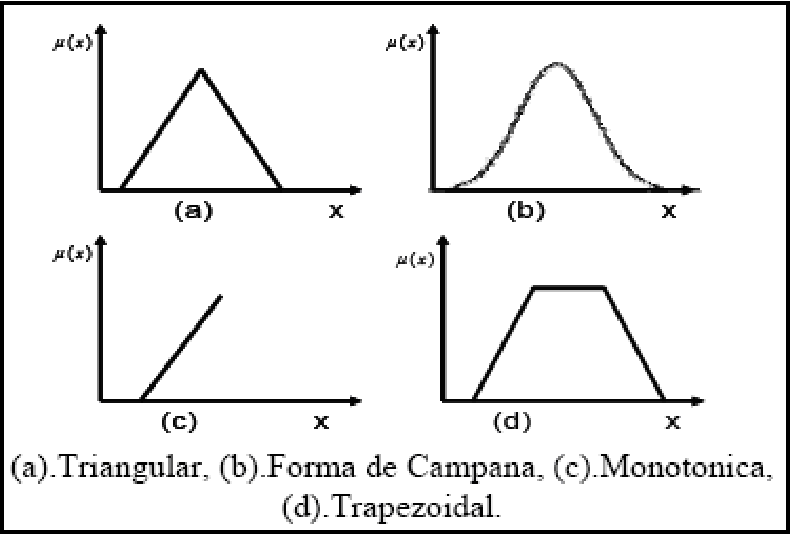
\includegraphics[width=0.5\linewidth]{\funcionM}
        \caption{Funciones de membresia mas comunes.}
        \label{fig:funcionM}
    \end{figure}

    \subsection{Fuzzificación}
    El control difuso siempre involucra este proceso de Fuzzificación, esta operación se realiza en todo instante de tiempo, es la puerta de entrada al sistema de inferencia difusa. Es un procedimiento matemático en el que se convierte un elemento del universo de discurso(variable medida del proceso) en un valor en cada función de membresía a las cuales pertenece.

    \begin{figure}[H]
        \centering
        \includegraphics[width=0.8\linewidth]{\fuzzy}
        \caption{Fuzzificación de una variable.}
        \label{fig:fuzzyV}
    \end{figure}

    Para comprender mejor veamos la figura~\ref{fig:fuzzyV} que arroja los siguientes datos:

    \begin{align}
        \mu_{\text{BAJOS}}(55) &= 0.25 \\
        \mu_{\text{REGULAR}}(55) &= 0.75 \\
        \mu_{\text{ALTOS}}(55) &= 0.00
    \end{align}

    El valor de velocidad igual a 55 pertenece a dos conjuntos con distintos grados en cada uno.
    A partir de ahora y durante el resto de las operaciones en el interior del corazón fuzzy estos datos (0.25, 0.75 y 0.00, son valores de las funciones de membresía) representarán a las variables censados del proceso. A tales datos les llamaremos $\mu$ en sentido genérico para diferenciarlos de otras funciones de membresía $\mu_A(x) = \mu$.


    \subsection{Mamdani.}
    Las reglas difusas de Mamdani son esenciales en sistemas de lógica difusa y controladores borrosos, modelando decisiones en entornos con imprecisión. Siguiendo la estructura "si-entonces", expresan condiciones y acciones en términos lingüísticos como "bajo" o "alto". Cada variable lingüística tiene funciones de membresía asociadas. Operaciones borrosas como "y" y "o" combinan condiciones en reglas ponderadas por su activación, definiendo el conocimiento del sistema. La inferencia difusa calcula la salida ponderadamente, y la defusificación convierte la salida difusa en un valor concreto para acciones. Estas reglas son versátiles, aplicándose en control difuso y toma de decisiones en contextos desafiantes para la precisión convencional.

    \subsection{defusificación.}
    La defusificación es la etapa crucial en un sistema de lógica difusa donde la salida difusa, expresada en conjuntos difusos, se convierte en un valor concreto para la toma de decisiones. Después de la inferencia difusa, que produce conjuntos difusos de salida, la defusificación busca resumir esta información en un valor numérico. Métodos comunes incluyen el uso del centro de gravedad, que encuentra el punto central ponderando los valores de salida por sus grados de membresía, y el método del valor máximo, que selecciona el valor máximo del conjunto difuso de salida como el resultado. La elección del método depende del contexto de la aplicación y los requisitos de precisión, siendo la defusificación esencial para traducir la información difusa en acciones o valores concretos en aplicaciones prácticas.



    
    \section{Metodología.}
    La metodología de este sistema es poco complicada, teniendo un grado de mayor dificultad proporcionar las salidas y entradas correctas para enlazar los código entre los módulos para una única salida.
    Abordando los módulos en el orden que me parece adecuado, podemos considerara que se requiere realizar un prescaler para que los cambios del reloj al leer los pulsos no sean muy rápidos, lo cual nos da la holgura necesaria en los módulos para leer de manera correcta todas las señales, generando las salidas de una manera satisfactoria. El módulo de “anti-rebote” obtiene mediante el módulo principal SYSTEM unos retrasos, que se verifican en el módulo de pulsos de reloj, el cual tiene como función principal, asegurarse de que los 3 retrasos se den sobre el reloj del preescaler, así los botones utilizados para las entradas quedan condicionados,  para que solo un señal de pulso se tome en cuenta, pasando el primer pulso entre los 3 retrasos, además se condiciona esta salida para verificar que todos sean iguales, generando de manera satisfactoria un solo pulso desde los botones de entrada, también en este módulo es donde se realiza la codificación, ya que se pasan los valores de los botones a los valores que utilizaremos  sobre el código final.
    Contamos con el módulo de las máquinas de estado que es donde se manejan las situaciones posible en base al diseño principal como en la figura~\ref{fig:estados}, el cual consiste en colocar  digamos 2 “caminos” diferentes por lo cuales se puede llegar a una salida, esto debido a el planteamiento del problema donde se requiere que la salida se de hasta tener las 4 iteraciones que requiere el dígito para ser correcto, que si se considera, esto tiene sentido ya que al ser un sistema de seguridad no debería de dar pista de donde están los errores, así que se limita a tener una salida de \emph{aprobado} o \emph{fallo} en cada iteración completa del sistema, así que si pasamos por los estados $ \{q_0,q_1,q_2,q_3\} $ generamos un valor correcto y obtendremos una señal de \emph{aprobado}, mientras que si erramos algun digito, podemos pasar por los estados $\{q_4,q_5,q_6\}$, que manejan los errores para completar la iteración de 4 digitos, así mismo tenemos una particularidad que es que los valores intermedios pasan del camino correcto al manejo de errores en los estados $\{q_0,q_1,q_2\}$, pero en el estado $q_3$, el error se maneja sobre el mismo estado dando salida a diferentes valores, si el codigo es correcto activaremso la señal de \emph{aprobado}, mientras que si el codigo esta mal sobre ese ultimo dígito daremos paso a  la salida de \emph{fallo} , por ultimo como se dijo el modulo de \emph{system}, une las señales pasando el reloj principal al preescaler, la salida de este modulo al modulo de pulsos e reloj, que a su vez da parte de las entradas al modulo de entirrebote, tambien se pasan los valores de los botones pulsados, asegurando la lectura de un solo valor y pasando los valores de estos a el modulo de las maquinas de estado, el cual como se dijo da paso a la señales aprobado o fallo, dichas señales se puede interpretar de manera fisica sobre la tarjeta al ver el $led_0$ para fallo y $led_1$ para aprobado, el valor del codigo a verificar es determinado por el vector \emph{secret\_code} que se lee sobre este mismo modulo. dicho valor se obtiene a través de los switch 0 a 7 de la tarjeta \emph{Basys 3}.


    \section{Análisis de resultados.}
	Una vez establecido el diseño, los conjuntos y las reglas para el controlador se realizan los cálculos necesarios para obtener los valores de pertenencia, con estos y usando las reglas del controlador podemos obtener los resultados de salida.
	\begin{figure}[!h]
		\centering
		\includegraphics[scale=0.5]{\imgA}
		\caption{Gráfico en el comportamiento del controlador difuso.}
	\end{figure}
	Por cada una de las reglas se van analizando las relaciones de pertenencia a las que corresponden sus respectivas entradas y estas se van uniendo en la gráfica final en la que se obtendrá la figura final y en ella se tomará su centroide el cual será la salida a sus correspondientes dispositivos.\newline \\
	Con ayuda de la gráfica se aprecia que las salidas del controlador se van adaptando cada vez que se hace un cambio de modo que se obtiene de forma automática un valor adecuado según cada situación.\newline \\
	En el siguiente gráfico se observa como el controlador va tomando los valores de entrada tras calcular los valores de pertenencia determina en que situación se encuentra el entorno de modo que puede aumentar la apertura de las persianas para captar más luz además de determinar que la temperatura es adecuada por lo que buscará mantenerla en el mismo valor.
	\begin{figure}[!h]
		\centering
		\includegraphics[scale=0.5]{\imgB}
		\caption{Resultados al tomar entradas de poca luz y a baja temperatura.}
	\end{figure}
    

    \section{Conclusión}
    Este proyecto ha logrado el objetivo de crear un sistema de control de acceso seguro y eficiente mediante la combinación de VHDL en Vivado. Aunque la metodología puede parecer compleja en un principio, la modularidad de los componentes ha facilitado su desarrollo, así como el mantenimiento que se le pueda dar. Además, el sistema se ha diseñado teniendo en cuenta la seguridad y la usabilidad, lo que puede llevarlo a escalar a una solución sólida para el control de acceso a una puerta con código secreto. Como futuras mejoras, se podrían explorar posibilidades de la integración con sistemas de control más amplios, hemos logrado desarrollar un diseño modular, cuya estructura de módulos, que incluye el prescaler, el anti-rebote y las máquinas de estado, ha demostrado ser altamente efectiva en el manejo de las señales de entrada, así como en la generación de salidas adecuadas que podemos verificar mediante los diagramas de tiempos obtenidos de la simulación, también la implementación de la lógica de codificación asegura una comparación precisa con el código secreto, mediante la configuración que se pueda dar mediante los switch. La retroalimentación visual mediante LED simplifica la interacción con el sistema. La gestión de errores y la separación de caminos para aprobación y fallo mejoran aún más la seguridad, ya que como se comentó, esto deja sin pistas de donde está en el error, si bien el sistema es pequeño se puede considerar que, teniendo esto como base se podría desarrollar un sistema más robusto bajo la misma línea de pensamiento, cosa que dependiendo de la metodología de desarrollo que se tenga puede cambiar o no, que en lo personal creo que cambiaria, pero seria interesante ver cuales son esos cambios a efectuar sobre el sistema y como la mayoría de cosas en ingenieria, saber que tanto estábamos cerca de algo viable o no.   



    % \begin{figure}[H]
    %     \centering
    %     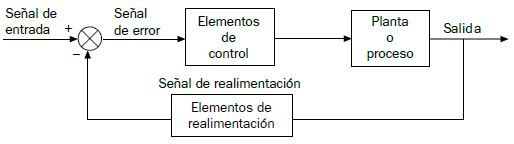
\includegraphics[width=\textwidth,height=10cm, keepaspectratio]{\control}
    %     \caption{Diagrama a bloques de lazo cerrado}
    %     \label{fig:control}
    % \end{figure}

    
\end{document}
